\documentclass[a4j]{jsarticle}
\usepackage[dvipdfmx]{graphicx}
\usepackage{float}

\title{RSA暗号の暗号化}
\author{C0118005 秋本 遥基}
\date{2019/06/10}

\begin{document}
\maketitle

\section{はじめに}
本レポートはRSA暗号による暗号手順について考察をするものである。

\section{RSA暗号による暗号化および復号}
RSA暗号による暗号化及び復号の手順を実例を用いて示す。

\subsection{初期値の設定}
平文mを設定する。

\begin{eqnarray}
  学籍番号はC0118005\\
  n &=& pq \\
  n &=& 19 \times 31\\
  &=& 589\\
  118005 \div (589-2) &=& 201 \dots 18\\
  m &=& 18 + 2\\
  &=& 20 
\end{eqnarray}

今回は学籍番号の数字部分をn-2で割りその余りに2を足した数で生成する。
RSA暗号は2数の素数を用いるが今回はこれを$p,q &=& 19,31$とする。
また、nはこの2数の積によって求められる。
したがって、$n &=& 19 \times 31$より $n &=& 589$となる。
また$n-2$より、割る値は$587$となる。
$ 118005 \bmod 587 &=& 18$
よって$m &=& 18+2 &=& 20$

\subsection{秘密鍵および公開鍵の設定}

以下の式により、秘密鍵d、公開鍵e及びnを設定する。

\begin{eqnarray}
  \label{LCM}
  \lambda(n) &=& LCM(p-1, q-1)\\
  \label{GCD}
  GCD(e,\lambda_{(n)}) &=& 1  (e \in \mathbb{Z}_{\lambda(n)})\\
  \label{d}
  d &=& \frac{1}{e} \bmod {\lambda(n)} 
\end{eqnarray}

(\ref{LCM})のLCM()は関数内の最小公倍数を返すものである。
したがって、p-1=18,q-1=30の最小公倍数であり、これは90である。

(\ref{GCD})のGCD()は関数内の最大公約数を返すものである。
したがって、これは最大公約数が1となるためeと\lambda(n)は互いに素な関係である。
これを満たすeは、\lambda(n)と素でありかつ0以上\lambda(n)未満な数である。
よってeの候補は{7,11,13,17,19,23,29,31,37,41,43,47,53,59,61,67,71,73,79,83,89}である。

次に(\ref{d})を求める。
ここでeを7とすると、7d-1が\lambda(n)で割り切れるものを探せば良いので、
d = 13がこれに該当する。
したがって、d = 13,e = 7,n = 589, m = 20となる。

\subsection{暗号化と復号}
\begin{eqnarray}
 \label{c}
 c = m^e \bmod n\\
 \label{rm}
 m = c^d \bmod n 
\end{eqnarray}

ここでは、前節で設定した値を用いて暗号化をする。
また、暗号文をcと定める。
暗号文はで(\ref{c})求められる。
したがって、これはm=20のe=7乗をn=589で割ったあまりであり、514となる。
この計算を以下の図に示す。

\begin{figure}[H]
  \centering
  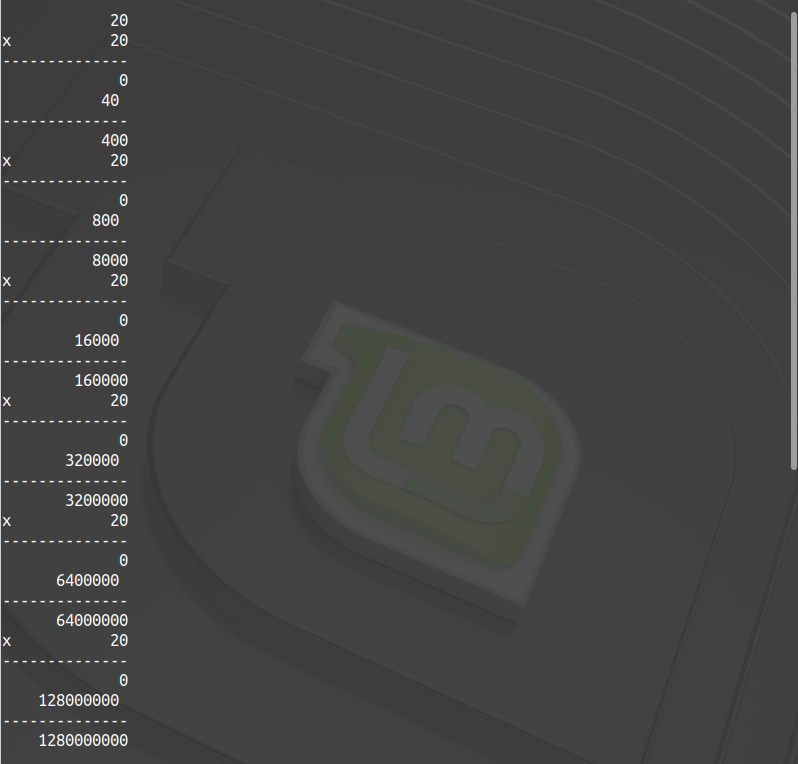
\includegraphics[scale = 0.50]{hissan03.png}
  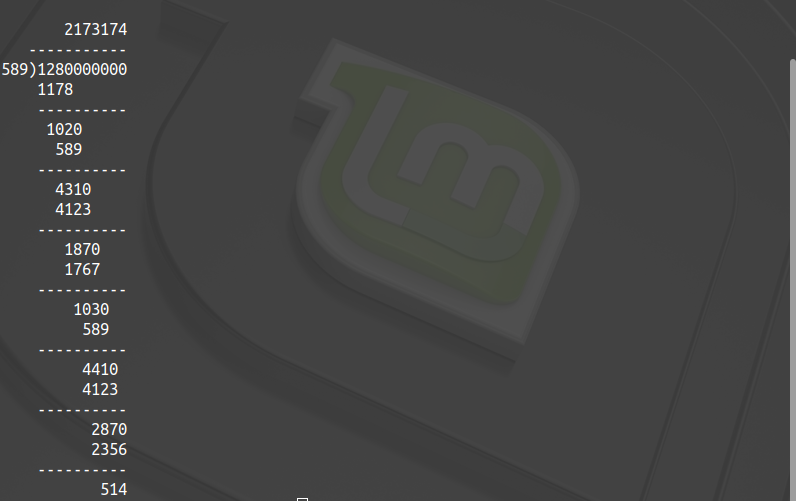
\includegraphics[scale = 0.50]{hissan04.png}
  \caption{$m^e \bmod n$の筆算}
  \label{figure:m^e}
\end{figure}

また、この復号は(\ref{rm})で求められる。
これは20となり、正しく復号されたことがわかる。
この計算を以下の図に示す。

\begin{figure}[H]
  \centering
  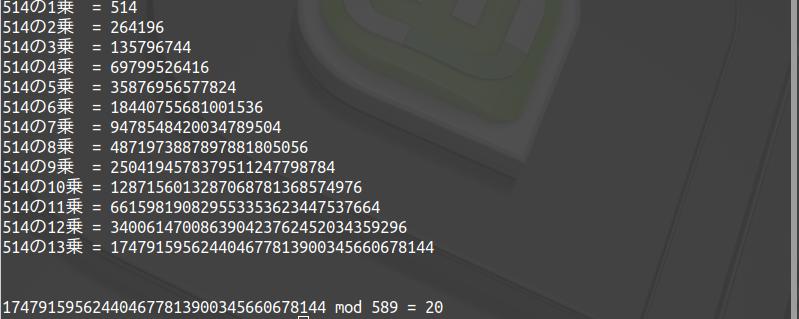
\includegraphics[scale = 0.50]{hissan05.png}
  \caption{$c^d \bmod n$の筆算}
  \label{figure:c^d}
\end{figure}

\section{考察}

RSA暗号による暗号のnを決めるための2値の推定の難しさと、
公開鍵と秘密鍵による暗号化・復号の容易さが確かめられた。

また、素因数分解とpとqの長さによる難解さであり2002年時点でのnの推奨サイズは1024ビット、
すなわちp、qの長さはおおよそ512ビットとなる。

\end{document}
